% Options for packages loaded elsewhere
\PassOptionsToPackage{unicode}{hyperref}
\PassOptionsToPackage{hyphens}{url}
%
\documentclass[
  letterpaper,
  ignorenonframetext,
  aspectratio=43,
  handout,
  12pt]{beamer}
\usepackage{pgfpages}
\setbeamertemplate{caption}[numbered]
\setbeamertemplate{caption label separator}{: }
\setbeamercolor{caption name}{fg=normal text.fg}
\beamertemplatenavigationsymbolsempty
% Prevent slide breaks in the middle of a paragraph
\widowpenalties 1 10000
\raggedbottom
\setbeamertemplate{part page}{
  \centering
  \begin{beamercolorbox}[sep=16pt,center]{part title}
    \usebeamerfont{part title}\insertpart\par
  \end{beamercolorbox}
}
\setbeamertemplate{section page}{
  \centering
  \begin{beamercolorbox}[sep=12pt,center]{part title}
    \usebeamerfont{section title}\insertsection\par
  \end{beamercolorbox}
}
\setbeamertemplate{subsection page}{
  \centering
  \begin{beamercolorbox}[sep=8pt,center]{part title}
    \usebeamerfont{subsection title}\insertsubsection\par
  \end{beamercolorbox}
}
\AtBeginPart{
  \frame{\partpage}
}
\AtBeginSection{
  \ifbibliography
  \else
    \frame{\sectionpage}
  \fi
}
\AtBeginSubsection{
  \frame{\subsectionpage}
}
\usepackage{amsmath,amssymb}
\usepackage{lmodern}
\usepackage{ifxetex,ifluatex}
\ifnum 0\ifxetex 1\fi\ifluatex 1\fi=0 % if pdftex
  \usepackage[T1]{fontenc}
  \usepackage[utf8]{inputenc}
  \usepackage{textcomp} % provide euro and other symbols
\else % if luatex or xetex
  \usepackage{unicode-math}
  \defaultfontfeatures{Scale=MatchLowercase}
  \defaultfontfeatures[\rmfamily]{Ligatures=TeX,Scale=1}
\fi
\usetheme[]{metropolis}
% Use upquote if available, for straight quotes in verbatim environments
\IfFileExists{upquote.sty}{\usepackage{upquote}}{}
\IfFileExists{microtype.sty}{% use microtype if available
  \usepackage[]{microtype}
  \UseMicrotypeSet[protrusion]{basicmath} % disable protrusion for tt fonts
}{}
\makeatletter
\@ifundefined{KOMAClassName}{% if non-KOMA class
  \IfFileExists{parskip.sty}{%
    \usepackage{parskip}
  }{% else
    \setlength{\parindent}{0pt}
    \setlength{\parskip}{6pt plus 2pt minus 1pt}}
}{% if KOMA class
  \KOMAoptions{parskip=half}}
\makeatother
\usepackage{xcolor}
\IfFileExists{xurl.sty}{\usepackage{xurl}}{} % add URL line breaks if available
\IfFileExists{bookmark.sty}{\usepackage{bookmark}}{\usepackage{hyperref}}
\hypersetup{
  hidelinks,
  pdfcreator={LaTeX via pandoc}}
\urlstyle{same} % disable monospaced font for URLs
\newif\ifbibliography
\usepackage{graphicx}
\makeatletter
\def\maxwidth{\ifdim\Gin@nat@width>\linewidth\linewidth\else\Gin@nat@width\fi}
\def\maxheight{\ifdim\Gin@nat@height>\textheight\textheight\else\Gin@nat@height\fi}
\makeatother
% Scale images if necessary, so that they will not overflow the page
% margins by default, and it is still possible to overwrite the defaults
% using explicit options in \includegraphics[width, height, ...]{}
\setkeys{Gin}{width=\maxwidth,height=\maxheight,keepaspectratio}
% Set default figure placement to htbp
\makeatletter
\def\fps@figure{htbp}
\makeatother
% Make links footnotes instead of hotlinks:
\DeclareRobustCommand{\href}[2]{#2\footnote{\url{#1}}}
\setlength{\emergencystretch}{3em} % prevent overfull lines
\providecommand{\tightlist}{%
  \setlength{\itemsep}{0pt}\setlength{\parskip}{0pt}}
\setcounter{secnumdepth}{-\maxdimen} % remove section numbering
\usepackage{pgfpages}
\pgfpagesuselayout{2 on 1}
\providecommand{\tightlist}{%
\setlength{\itemsep}{0pt}\setlength{\parskip}{0pt}}
\makeatletter
\makeatother
\let\Oldincludegraphics\includegraphics
\renewcommand{\includegraphics}[2][]{\Oldincludegraphics[width=\textwidth,height=0.7\textheight,keepaspectratio]{#2}}
\ifluatex
  \usepackage{selnolig}  % disable illegal ligatures
\fi

\author{}
\date{}

\begin{document}

\begin{frame}{AE 737: Mechanics of Damage Tolerance}
\protect\hypertarget{ae-737-mechanics-of-damage-tolerance}{}
Lecture 10 - Residual Strength

Dr.~Nicholas Smith

Wichita State University, Department of Aerospace Engineering

3 March, 2021
\end{frame}

\begin{frame}{schedule}
\protect\hypertarget{schedule}{}
\begin{itemize}
\tightlist
\item
  3 Mar - Residual Strength
\item
  5 Mar - HW4 Due, HW 3 Self-grade due
\item
  8 Mar - Multiple Site Damage
\item
  10 Mar - Mixed-Mode Fracture
\item
  12 Mar - HW5 Due, HW4 Self-grade due
\end{itemize}
\end{frame}

\begin{frame}{outline}
\protect\hypertarget{outline}{}
\begin{itemize}
\tightlist
\item
  stiffeners
\item
  severed stiffeners
\item
  crack stoppers
\end{itemize}
\end{frame}

\hypertarget{stiffeners}{%
\section{stiffeners}\label{stiffeners}}

\begin{frame}{stiffened panels}
\protect\hypertarget{stiffened-panels}{}
\begin{itemize}
\tightlist
\item
  In aircraft the skin/stringer system provides many benefits
  (resistance to buckling)
\item
  Stringers also act as stiffeners to resist crack propagation in the
  skin
\item
  Panels in these configurations are generally very wide relative to
  expected crack dimensions
\item
  Cracks are generally modeled either as centered between stiffeners or
  centered under a stiffener
\item
  We need to consider the residual strength of the panel, the stiffener,
  and the rivets
\end{itemize}
\end{frame}

\begin{frame}{centered between stiffeners}
\protect\hypertarget{centered-between-stiffeners}{}
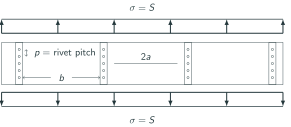
\includegraphics{../images/crack-under.svg}
\end{frame}

\begin{frame}{centered under stiffener}
\protect\hypertarget{centered-under-stiffener}{}
\includegraphics{../images/crack-between.svg}
\end{frame}

\begin{frame}{remote stress}
\protect\hypertarget{remote-stress}{}
\begin{itemize}
\tightlist
\item
  For displacement continuity, we know that
\end{itemize}

\[\left(\frac{PL}{AE}\right)_{Skin} = \left(\frac{PL}{AE}\right)_{Stiffener}\]

\begin{itemize}
\tightlist
\item
  Since \emph{L} is the same, we find
\end{itemize}

\[\frac{S}{E} = \frac{S_S}{E_S}\]

\begin{itemize}
\tightlist
\item
  Where the subscript \emph{S} indicates stiffener values, we can
  express the remote stress in the stiffener as
\end{itemize}

\[S_S = S \frac{E_S}{E}\]
\end{frame}

\begin{frame}{skin}
\protect\hypertarget{skin}{}
\begin{itemize}
\tightlist
\item
  The critical stress in the skin is determined the same way as it was
  in the residual strength chapter
\item
  The only exception is that the stiffener contributes to \(\beta\)
\end{itemize}

\[S_C = \frac{K_C}{\sqrt{\pi a} \beta}\]
\end{frame}

\begin{frame}{stiffener}
\protect\hypertarget{stiffener}{}
\begin{itemize}
\tightlist
\item
  The maximum stress in a stiffener will be increased near a crack
\item
  We represent the ratio of maximum force in stiffener to remote force
  with the Stiffener Load Factor, \emph{L}
\end{itemize}
\end{frame}

\begin{frame}{stiffener}
\protect\hypertarget{stiffener-1}{}
\[\small{\begin{aligned}
  L &= \frac{\text{max force in stiffener}}{\text{remote force applied to stiffener}}\\
  &= \frac{S_{S,max}A_S}{S_S A_S}\\
  &= \frac{S_{S,max}}{S \frac{E_S}{E}}\\
  L S \frac{E_S}{E} &= S_{S,max}\\
  L S \frac{E_S}{E} &= \sigma_{YS}\\
  S_C &= \frac{\sigma_{YS} E}{L E_S}
\end{aligned}}\]
\end{frame}

\begin{frame}{rivet}
\protect\hypertarget{rivet}{}
\begin{itemize}
\tightlist
\item
  We can define a similar rivet load factor to relate maximum stress in
  the rivet to remote stress in the skin
\end{itemize}

\[\begin{aligned}
  L_R &= \frac{\tau_{max} A_R}{S b t}\\
  L_R &= \frac{\tau_{YS} A_R}{S b t}\\
  S_c &= \frac{\tau_{YS} A_R}{L_R b t}
\end{aligned}\]
\end{frame}

\begin{frame}{finite element analysis}
\protect\hypertarget{finite-element-analysis}{}
\begin{itemize}
\tightlist
\item
  CC Poe found that panels could be related by a parameter he defines as
  \$\mu\$
\end{itemize}

\[\mu = \frac{A_S E_S}{A_S E_S + A E}\]

\begin{itemize}
\tightlist
\item
  Where \emph{A}\emph{S} is the cross-sectional area of a stiffener,
  \emph{E}\emph{S} is stiffener modulus
\item
  \emph{A} is the skin cross-sectional area (per stiffener)
  \emph{A}=\emph{bt} and \emph{E} is the modulus of the skin
\end{itemize}
\end{frame}

\begin{frame}{finite element analysis}
\protect\hypertarget{finite-element-analysis-1}{}
\begin{itemize}
\tightlist
\item
  pp 167 - 178 give \(\beta\) \emph{L} and \emph{L}\emph{R} for various
  skin/stiffener configurations
\item
  These values were determined using a finite element model
\end{itemize}
\end{frame}

\begin{frame}{examples}
\protect\hypertarget{examples}{}
\begin{itemize}
\tightlist
\item
  quantitative example (p.~179-180)
\item
  qualitative notes on behavior (p.~181-182)
\item
  \href{../examples/stiffener\%20example.html}{worked}
\end{itemize}
\end{frame}

\hypertarget{severed-stiffeners}{%
\section{severed stiffeners}\label{severed-stiffeners}}

\begin{frame}{failure in stiffener}
\protect\hypertarget{failure-in-stiffener}{}
\begin{itemize}
\tightlist
\item
  Sometimes the stiffeners fail before the panel
\item
  T. Swift conducted some parametric studies on panels with a severed
  stiffener
\item
  When the crack is short (and near the severed stiffener) the residual
  strength is lower due to the broken stiffener
\item
  As the crack nears the next stiffener, residual strength is very
  similar to a panel with all stiffeners intact
\end{itemize}
\end{frame}

\begin{frame}{failure in stiffener}
\protect\hypertarget{failure-in-stiffener-1}{}
\begin{itemize}
\tightlist
\item
  Swift considers the difference in stress at different points in the
  stiffener
\item
  Instead of one general load factor (\emph{L}), he uses \emph{SCFO} and
  \emph{SCFI}
\item
  We can find the critical value of remote stress at the outer flange as
\end{itemize}

\[\sigma_C = \frac{\sigma_U}{SCFO}\]

\begin{itemize}
\tightlist
\item
  And similarly at the inner flange
\end{itemize}

\[\sigma_C = \frac{\sigma_U}{SCFI}\]

\begin{itemize}
\tightlist
\item
  Swift's parametric study did not consider rivet failure
\end{itemize}
\end{frame}

\begin{frame}{stiffener area}
\protect\hypertarget{stiffener-area}{}
\includegraphics{../images/stiffener_area.jpg}
\end{frame}

\begin{frame}{stiffener spacing}
\protect\hypertarget{stiffener-spacing}{}
\includegraphics{../images/stiffener_spacing.jpg}
\end{frame}

\begin{frame}{rivet spacing}
\protect\hypertarget{rivet-spacing}{}
\includegraphics{../images/rivet_spacing.jpg}
\end{frame}

\begin{frame}{strength and toughness increase}
\protect\hypertarget{strength-and-toughness-increase}{}
\includegraphics{../images/strength_increase.jpg}
\end{frame}

\begin{frame}{example}
\protect\hypertarget{example}{}
\begin{itemize}
\tightlist
\item
  If we consider the case from Swift's data most similar to our previous
  example:
\end{itemize}

\[\begin{aligned}
  P &= 1.0 \text{ in}\\
  A_{st} &= 0.2538 \text{ in}^2\\
  b &= 10.0 \text{ in}\\
\end{aligned}\]

\begin{itemize}
\tightlist
\item
  So we use the tables for Case 10
\end{itemize}
\end{frame}

\hypertarget{crack-stoppers}{%
\section{crack stoppers}\label{crack-stoppers}}

\begin{frame}{crack stopper}
\protect\hypertarget{crack-stopper}{}
\includegraphics{../images/crack_stoppers.jpg}
\end{frame}

\begin{frame}{optimal crack stopper}
\protect\hypertarget{optimal-crack-stopper}{}
\begin{itemize}
\tightlist
\item
  Swift found that the ideal crack stopper has a cross-sectional area
  approximately equal to 1/4 the stiffener area
\item
  The ideal material was titanium (as opposed to steel or aluminum).
\item
  Aluminum did not transfer enough load to the stiffeners, steel
  transferred too much
\end{itemize}
\end{frame}

\begin{frame}{example}
\protect\hypertarget{example-1}{}
\begin{itemize}
\tightlist
\item
  Compare cases 1, 3, and 5
\end{itemize}
\end{frame}

\end{document}
